\chapter{Nanopores: beyond DNA sequencing}
\label{chapter_6}


\blfootnote{This chapter is based on a manuscript in preparation as: Y. Ying, Z. Hu, S. Zhang, Y. Qing, A. Fragasso, X. Zhang, G. Maglia, A. Meller, H. Bayley,C. Dekker, L. Jiang, Y. Long. Nanopores: Beyond DNA Sequencing.}
%% The following annotation is customary for chapter which have already been
%% published as a paper.
%\blfootnote{This chapter has been published as: }

%% It is only necessary to list the authors if multiple people contributed
%% significantly to the chapter.
%\authors{Albert {\titleshape Einstein}}
%
%%% The '0pt' option ensures that no extra vertical space follows this epigraph,
%%% since there is another epigraph after it.
%\epigraph[0pt]{
%    Nature and nature's laws lay hid in the night; \\
%    God said `Let Newton be!' and all was light.
%}{Alexander Pope}
%
%\epigraph{
%    It did not last: the devil shouting `Ho. \\
%    Let Einstein be!' restore the status quo.
%}{Sir John Collings Squire}

\begin{abstract}
The biological cell is full of many types of nanopores that govern the passage of individual molecules. Leaning from nature, nanopore techniques have developed into the ultimate analytical tool for sensing single molecules. Nanopore-based single-molecule DNA sequencing has propelled genomic science with improved sensitivity, lower costs, and long reads. Notably however, the sensing capabilities of the unique nanopore technique extend well beyond DNA sequencing. Here, we offer a comprehensive review that illuminates nanopore applications beyond DNA sequencing, with clear prospects for protein analysis and sequencing, single-molecule covalent chemistry, single-molecule liquid biopsy, and biomimetic pore engineering for understanding natural systems. These developments showcase nanopores as a general tool for biophysics, bioinformatics, and cheminformatics. 



\end{abstract}
\newpage


\section{Introduction}
Nanopores are an emerging class of single-molecule biosensors which have been developed primarily for ultra-sensitive DNA sequencing, as well as for other label-free biomol\-ecular sensing. Nanopores can be formed by several ways: biological nanopores are formed by self-assembly of either protein sub-units, peptides or even DNAs scaffold in lipid bilayers or in block copolymer membranes. Solid-state nanopores are crafted in freely suspended thin membrane by a variety of nanoscale milling tools including electron/ion/laser beam drilling, by la\-ser-based optical-etching method, or using dielectric breakdown of ultrathin solid membranes \cite{Varongchayakul2018,Ying2018,Restrepo-Perez2018,McGinn2016}. Alternatively, nanopores can be formed by controlled pulling of glass capillaries in designated instruments \cite{Yu2019}. 


Nanopores provides a geometric confinement to molecules that are temporarily lo\-dged in its interior volume, to allow label free sensing. Additionally, nanopores may offer a controllable chemical environment for single molecules and ions used to facilitate chemical reactions in this nanoscale volume. Both features may be utilized for single-molecule manipulation and sensing. In the most common nanopore measurement, the individual analyte is inserted inside the nanopore under applied potentials, hence altering the physical free flow of ions through the nanopore and permitting a straightforward temporal Ohmic measurement. Ideally, the geometry of the nanopore should be comparable to that of the analyte, to produce a significant change in the ion current amplitude from the presence of the analyte above the noise level. Additionally, a tight fit between the nanopore and analyte enhances the interactions between them, which accounts for the overall sensitivity and selectivity of the device \cite{Meller2003}. The size, shape and chemical properties of the nanopore could be tuned and manipulated at nanometer to subnanometer scale to further enhance its properties. For example, site-direct mutagenesis of protein nanopores may contribute to optimal interactions in nanopore confinement for specific analyte recognitions. This feature allows nanopore to controllably capture, identify, and transport any molecules and ions from the bulk solution. 


Nanopore sensors were initially used to stochastically characterize single molecules in a relatively simple, high-throughput, label-free format. By analyzing modulations of the ionic current in blockade amplitude, duration and frequency, nanopores have applied to sense and characterize a vast range of molecules, including DNAs, messenger and transfer RNAs, peptides, proteins, protein-DNA complexes and even metabolites \cite{Liu2021,Cao2016,Galenkamp2018,Zhang2017,Wanunu2010,Nir2015,Squires2015a,Depledge2019}. Today, the success of nanopore-based DNA sequencing has stimulated potential applications in many fields.


Although DNA sequencing has been the main focus for the nanopore method in the past two decades, the technique currently extends well beyond sequencing, as it hass been adapted to analyze molecular heterogeneities and stochastic processes in many different biochemical systems with single-molecule precision. This is due to a number of factors. First, a key advantage of nanopores lies in its ability to successively capture many single molecules one after the other at relatively high rate. This feature permits nanopores to explore large populations of molecules at single-molecule level in reasonable timeframes to understand their properties and dynamic behavior. Consequently, nanopores can be used to gain new molecular and mechanistic insights in a broad spectrum of molecular biosystems. 
\begin{figure}[!htbp]
	\centering
	\includegraphics[width=1\linewidth]{figures/Figure6.1.pdf}
	\caption{Nanopore techniques beyond DNA sequencing. The figure illustrates five areas of research where nanopores have great potential to contribute to new knowledge and new technologies.}
	\label{fig:fig6.1}
\end{figure}
Second, as nanopores essentially convert structural and chemical properties of the analytes into a measurable ion current signal, the nanopore can be used to report on multiple molecular features while circumventing the use of labelling chemistries, which complicate the analysis process and may affect the molecular structures. For example, recent studies showed that nanopore could discriminate 13 amino acids in a label-free manner, including some minute structural differences \cite{Ouldali2020}. An important aspect is the ability of nanopores to identify rare or aberrant species, which lack suitable labels for the signal amplification or whose information are hidden in the noise of analytical devices. Consequently, the nanopore may serve well in molecular diagnostic applications required for precision medicine, which make use of protein analyses, as well as other biomarker identification. Third, nanopores provide a well-defined scaffold to controllably design and construct biomimetic systems, which involve complex network of biomolecular interactions. These nanopore systems may be used to study the binding dynamics of transport biomolecules as they interact with the nanopore surfaces, hence serving as a sophisticated platform for unraveling complex biological processes \cite{Fragasso2021,Li2021}. Forth, chemical groups can be spatially aligned along the sensing interface of the protein nanopore, providing a sterically confined chemical environment for site-selective or regioselective covalent chemistry. This strategy has been used to engineer biological nanopores to serve as nanoreactors for the analysis of single-molecule reactions, such as the making and breaking of disulfide bonds \cite{Qing2018a,Qing2019}.


In this review paper, we discuss the state of the art in current nanopore research, as well as opportunities and the main challenges for the next decade, as the field shifts beyond DNA sequencing applications. We specifically address emerging nanopore methods for protein analysis and protein sequencing, single-molecule liquid biopsy, single-molecule covalent chemistry, and insights of biomimetic pores in analyzing complex biological processes.



\section[Characterization of single proteins with nanopores]{Characterization of single proteins with \\nanopores}
After the spectacular success following the sequencing of nucleic acids by nanopores, academic efforts are now shifting towards studying proteins. As an organism such as ourselves exhibits millions of different proteins, the challenge in proteomics involve identifying proteins, quantifying their abundance, and characterizing the choreography of post translational modifications that underlie their function. Several approaches to protein identifications are being explored.


Folded proteins have been sensed using solid-state \cite{Firnkes2010} and biological \cite{Soskine2012} nanopores. Properties such as protein volume, dipole and shape can be inferred by analyzing the translocation dynamics of proteins through nanopores \cite{Houghtaling2019}, indicating that nanopores are useful for extracting generic properties of proteins. Alternatively, ligands such as biotin \cite{Movileanu2000}, aptamers \cite{Rotem2012}, protein domains \cite{Thakur2019}, or antibodies \cite{Fahie2015} directly attached to nanopores or ligands attached to DNA carriers have been used to identify specific proteins (Fig. \ref{fig:fig6.2}a), even in the presence of complex media such as serum \cite{Chuah2019}. Beyond characterizing single proteins, nanopore arrays or specific fractionation protocols will be required to address the complexity of a proteome.

\begin{figure}[!htbp]
	\centering
	\includegraphics[width=1\linewidth]{figures/Figure6.2.pdf}
	\caption{Unravelling proteins with nanopores. a, Identification of streptavidin with $\alpha$-hemolysin ($\alpha$-HL) nanopore covalently modified with a PEG-biotin (top) as observed by a reduction of current noise (bottom) \cite{Movileanu2000}. b, Schematic of a single-molecule identifier in which a protein (\emph{e.g.} GFP, dark green) is fed to an unfoldase (purple) into peptidase (\emph{e.g.} proteasome, green and orange) attached to a nanopore (cyan) \cite{Zhang2020}. An idealized peptide fragmentation pattern is depicted (bottom). c, Unfolded transport of a construct including Smt3 (light green), GFP (dark green), and titin (cyan) – previously electrophoretic captured using a peptide thread (yellow) - through a nanopore operated by ClpXP (blue and red)(top). The unfolded translocation is shown in the electrical signal (bottom) \cite{Nivala2014}. d, Catalytic activity of DHFR (colored according to the vacuum electrostatics) inside ClyA nanopores (grey) (top), as shown by a representative traces (bottom). The formation of the product is shown by a pink asterisk \cite{Galenkamp2020b}. e, Immobilization of a protein (blue) inside a nanopore (grey) using a DNA-origami sphere (red) in the NEOtrap \cite{Schmid2021a}. The current trace indicates a trapping time of several hours. f, Dynamic conformation of a single peptide confined in a SiN\textsubscript{x} solid-state nanopore. The $\beta$-hairpin peptide was bound to a monovalent streptavidin (mSA). The ionic current (bottom) reflects different conformations of the target peptide (top right) \cite{Liu2021}. Figures are adapted from the indicated references.}
	\label{fig:fig6.2}
\end{figure}

Work is underway to use nanopores to detect single peptides as an alternative to mass spectrometry, the workhorse of proteomic analysis. Following initial work with model peptides \cite{Sutherland2004} and their post-translational modifications \cite{Restrepo-Perez2019}, it has been reported that, as observed earlier for PEG molecules \cite{Robertson2007}, peptide signals relate to their volume \cite{Chavis2017} (hence to a first approximation to the peptide mass). Another important step was the realization that by lowering the pH to <$\sim$4, all peptides can be captured despite their chemical composition \cite{Huang2017a}. Based on peptide-volume recognition, a single-molecule protein identifier has been proposed, in which a protease is placed directly above a nanopore, and the fragmented peptides are sequentially read by a nanopore sensor (Fig. \ref{fig:fig6.2}b) \cite{Huang2019a}. Initial steps to integrate a peptidase with a nanopore have been made \cite{Zhang2020}.


The ideal approach to nanopore proteomics, however, would be \emph{de novo} protein sequencing, where proteins are unfolded, linearly translocated across a nanopore amino acid by amino acid, and individual amino acids recognized by specific current signatures. Among the many challenges in such a \emph{de novo} sequencing, amino acid recognition appears tractable. Several laboratories could observe differences in single amino acids, on either peptides \cite{Ouldali2020} or stretched polypeptides \cite{Restrepo-Perez2019a}, and even differences between isomeric molecules have been reported \cite{Boersma2012}. Therefore, at least a subset of amino acids or post translational modifications should be addressable by nanopore currents. Attempts have also been made to control of the translocation of linearized proteins using unfoldases - enzymes that unfold protein using ATP as fuel. In a first example, transport was obtained using ClpXP which was used to pull on proteins pre-threaded through an $\alpha$-HL nanopore. The narrow entry of the nanopore was then used as a sieve to forcefully unfold the proteins (Fig. \ref{fig:fig6.2}c) \cite{Nivala2013}. Differences between proteins or modifications that affected the folded state of the protein have been reported \cite{Nivala2014}. Another approach used a proteolytically inactivated proteasome – a cylindrical multicomplex system that degrades proteins – genetically fused atop of a $\beta$-barrel nanopore \cite{Zhang2020}. The proteasome acted as a docking station for an unfoldase, which would then feed unfolded protein to the proteasome chamber and eventually through the nanopore. Both approaches require further developments, either to reduce the electrical signal generated by the unfolding process at the mouth of the nanopore \cite{Nivala2014}, or to control the stretching of the proteins as they translocate across the nanopore \cite{Zhang2020}. Recent work appears to provide a breakthrough towards protein sequencing, where a helicase was used to pull a DNA-peptide hybrid molecule through a nanopore in single amino acids steps, and single amino-acid substitutions were reliably detected within individual peptides \cite{Brinkerhoff2021}.


Beside identifying proteins, nanopores can be used as single-molecule sensors to characterize protein activity, dynamics, and conformational changes. Among the unique advantages of nanopores is the ability to sample native proteins at the single-molecule level with microsecond resolution with no intrinsic limitation on the observation period. In first implementations of nanopore enzymology, nanopores were used to monitor the formation of the product of bulk enzymatic reactions \cite{Kukwikila2015}, which might be useful when a straightforward spectroscopic assay is not available. However, this approach does not allow sampling the activities of individual enzymes. The latter has been first achieved by following the enzymatic ratcheting of a DNA strand across a nanopore \cite{Chu2010}, a method developed for DNA sequencing applications. For example, these studies revealed that Hel308 helicase moves a distance corresponding to half a DNA base during nucleotide binding and half a base during nucleotide hydrolysis, and that Phi29 DNA polymerase occasionally backsteps during amino acid incorporations \cite{Manrao2012}. Another approach has been to monitor the enzymes binding to the nanopore itself. Conformational changes of GroEL binding to a GroES-nanopore \cite{Chavis2017}, or kinases binding or phosphorylating a peptide introduced within the transmembrane region of a nanopore \cite{Cheley2006} have been observed. However, the relatively complex engineering of nanopores is likely to limit this approach to bespoke examples. 


A more generic approach is to temporarily trap a protein inside a nanopore. Conformational changes or dynamics can then be monitored through changes in the nanopore signal (Fig. \ref{fig:fig6.2}d-e). Proteins of 20-65 kDa can be captured by the electroosmotic flow within asymmetric biological nanopores, such as ClyA21 or PlyAB \cite{Huang2020a}, for variable periods. Importantly, at moderate voltages (<150 mV) no evidence of protein unfolding was observed \cite{Zernia2020}. Ligand-induced conformational changes for a range of proteins \cite{Galenkamp2020,VanMeervelt2017} have been reported. This included the tiny conformational changes of dihydrofolate reductase during ligand-binding \cite{Galenkamp2020} and catalysis \cite{Galenkamp2020b}, which previously could not be attained by single-molecule FRET studies \cite{Rajagopalan2002}. These studies revealed that DHFR exists in multiple fixed conformation – conformers –, which exchange during catalysis is most likely used to tune the enzyme’s efficiency \cite{Galenkamp2020,Galenkamp2020b}. Solid-state nanopores have also been used to sample proteins conformations \cite{Waduge2017}. However, the fast transport across the nanopores often prevents addressing multiple exchanges within single enzymes. This limitation has been addressed recently. In one example, a protein stopper was introduced to immobilize a biotinylated peptide inside a nanopore \cite{Liu2021}, allowing the measurement of multiple conformational exchanges. In another recent report a DNA lid was added to one side of a lipid-coated nanopore and proteins were added to the opposite side (Fig. \ref{fig:fig6.2}e-f) \cite{Schmid2021a}. The electrophoretic force allowed the DNA sphere to cover the nanopore, and the induced electroosmotic flow was used to trap a range of different proteins on the opposite side \cite{Schmid2021a}. Multiple conformational transitions of individual chaperone Hsp90 protein could be observed with this so-called NEOtrap.


\section{Single-Molecule Chemistry}
Single-molecule sensing generally involves non-covalent interactions \cite{Bayley2001}. Advances in this area suggested that covalent chemistry may be examined in a similar manner, and indeed bond making and bond breaking events of individual molecules attached to the interior wall of a nanopore can be analysed based on their modulation of the ionic current \cite{Bayley2008a}. Nanopores engineered to contain reactive sites are referred to as protein nanoreactors.


Examples include many aspects of the chemistry of thiols, introduced as cysteine side chains \cite{Steffensen2014}. Groups other than thiols can be examined after they have been introduced by site-directed chemical modification \cite{Ramsay2018a} or as non-canonical amino acids incorporated by native chemical ligation \cite{Lee2015}. The nanoreactor approach has been used to examine various aspects of photochemistry \cite{Luchian2003aSte}, to unravel the stereochemical course of transformations \cite{Steffensen2014}, to observe polymerization step-by-step \cite{Pulcu2019}, and to monitor a primary isotope effect \cite{Lu2010}. Catalytic cycles have been reconstituted by sampling partial reaction sequences in a nanopore after extricating intermediates from solution \cite{Ramsay2018} and reaction networks of considerable complexity that would be hard to deconvolute by say NMR have been disentangled \cite{Steffensen2014}.


The strengths and weaknesses of the nanoreactor approach to single-molecule covalent chemistry must be considered. On the plus side, no tagging of reactants is required. Because the pores formed by bacterial proteins are generally tough, a wide range of pH values, salt concentrations, and temperatures \cite{Kang2005} can be used. However, at this point, only aqueous chemistry has been examined. Both irreversible and reversible chemistry has been explored, and, because there are two compartments in a bilayer set up, incompatible spatially-separated reactants can be employed \cite{Luchian2003}. While attachment to the wall of the lumen is required to beat diffusion, it also prevents kinetic complications, such as the dimerisation of intermediates \cite{Lee2015}. If repeated turnover at a defined site is considered to be catalysis, examples have been observed \cite{Luchian2003}, but further progress on the use of nanopores to alter the course and rate of reactions is expected. Computer analysis of the frequency and lifetime of current states produces reaction schemes and kinetic constants for covalent chemistry with time resolution that can reach the 100-$\mu$s range \cite{Qing2018}. In general, standard deviations in rate constants are more than $\pm$5\%, which can be limiting, \emph{e.g.} only large isotope effects can be detected \cite{Lu2010}. While the nanoreactor approach provides a single-molecule reaction trajectory in which all steps are visible whether or not they are rate limiting \cite{Lu2010}, the molecular identification of intermediates can be problematic, as in any single-molecule approach. 


In early work, the kinetics of covalent chemistry within a nanoreactor were assumed to approximate the kinetics of ensemble reactions in bulk solution, and this is roughly correct for small molecules \cite{Bayley2008a}. More recently, interest has turned to considerations of how the environment within a nanopore, notably confinement, neighbouring groups, and chirality can affect chemistry, especially that of polymers, and how electrophoresis and electroosmosis \cite{Gu2003} can drive reactants into and out of pores. To enable chemistry on a polymer, its translocation through a nanoreactor can be arrested by either a terminal stopper protein or covalent linkage to the internal wall (Fig. \ref{fig:fig6.3}a). In the presence of a pulling force, imposed by either electrophoresis or electroosmosis \cite{Gu2003}, the polymer will extend and elongate within the tubular structure (Fig. \ref{fig:fig6.3}a). Additional force is exerted as the polymer emerges from confinement and regains conformational entropy (Fig. \ref{fig:fig6.3}a). Two features of nanopore confinement are advantageous for chemical manipulation. First, reactive groups spatially separated along the polymer chain can be aligned with inward-facing reactive side-chains. Second, the direction of the pulling force on a covalently-attached polymer, and thereby the polymer's orientation, can be switched by reversing the applied potential (Fig. \ref{fig:fig6.3}a), resetting the chemical landscape.


Alignment within a nanoreactor has been exploited to effect selective chemistry under confinement \cite{Qing2019}. As proof-of-concept, the interchange between disulfides within polymer backbones and cysteine thiols at different positions within a nanopore was examined (Fig. \ref{fig:fig6.3}b). The turnover of polymer substrates was enabled by using a competing small-molecule reductant (1,4-dithiothreitol, DTT, Fig. \ref{fig:fig6.3}b). Site selectivity was assessed as the fraction of a particular polymer that reacted at a particular location within a nanoreactor. The regioselectivity between two chemically equivalent sulfur atoms within a disulfide was determined by observing the characteristic currents associated with each reaction product (Fig. \ref{fig:fig6.3}b). Both site selectivity and regioselectivity showed strong dependences on the locations of cysteines in the nanopore and the disulfide in the polymer. This strategy might be adapted to other synthetic tubular nano-systems, such as metal-organic frameworks, to deliver site-selective or regioselective chemistry.


The selective chemistry promoted by confinement has been further elaborated into a processive molecular machine \cite{Astumian2012}, a ‘hopper’ which moves along a cysteine track within a nanopore while carrying a DNA cargo (Fig. \ref{fig:fig6.3}c) \cite{Qing2018a}. The hopper takes sub-nm steps through consecutive thiol-disulfide interchange reactions (Fig. \ref{fig:fig6.3}c). Reactions producing backward motion are strongly disfavoured when there is a pulling force on the DNA, endowing the hopper with remarkable directionality (Fig. \ref{fig:fig6.3}c). External control of the applied potential reorients the DNA within the nanopore and thereby resets the direction of hopping and the endpoint of the process (Fig. \ref{fig:fig6.3}c). Hopping is highly processive \cite{Qing2018a} and may provide a chemical alternative to the enzymatic ratchets used in sequencing technologies, which could be applied to polypeptides and polysaccharides as well as nucleic acids if longer tracks can be provided, for example on a patterned surface.


\begin{figure}[!htbp]
	\centering
	\includegraphics[width=1\linewidth]{figures/Figure6.3.pdf}
	\caption{Chemistry of polymers under confinement. a, Polymers, which coil in solution, are extended when confined within a tubular protein nanoreactor. This is achieved by non-covalently or covalently anchoring one end of the polymer and applying a pulling force, \emph{e.g.} an applied electric potential. In the case of covalent linkage, the polymer can be extended in either direction. b, Extending a polymer within a tubular nanoreactor exposes its reactive site (\emph{e.g.} a disulfide) to a reactive group positioned on the nanoreactor interior (\emph{e.g.} a cysteine thiol). In this way, spatial alignment differentiates between chemically equivalent reactive sites. Site selectivity and regioselectivity are determined at the single-molecule level by ionic current recording. The turnover of polymer substrates is enabled by 1,4-dithiothreitol (DTT). c, A molecular hopper moves along a multi-cysteine track under an applied potential while carrying a DNA cargo (green circles). Ratcheted by selective thiol-disulfide interchange reactions, the hopper makes steps in the direction of the pulling force. Real-time tracking of the hopper on track is achieved by monitoring the ionic current. Reversal of the applied potential flips the hopper, which then moves in the opposite direction.}
	\label{fig:fig6.3}
\end{figure}

\section{Synthetic nanopores as a tool to study biological questions}
While nanopores understandably attract most attention for their use in sequencing and bioanalytical applications, they also offer exciting opportunities to study questions that arise in cell biology. Cells feature a wide variety of nanometer-sized pores within their membranes (Fig. \ref{fig:fig6.4}a), that act as gateways for molecular transport between compartments. For example, the flow of ions and small molecules (\emph{e.g.} ATP) is regulated by ion channels and transporters, with crucial roles in homoeostasis, energy production, cellular communication, and sensory transduction \cite{DalePurvesGeorgeJ.AugustineDavidFitzpatrickLawrenceC.KatzAnthony-SamuelLaMantiaJamesO.McNamara2001}. Larger pores, such as the mitochondrial translocase \cite{Dekker1998} and the nuclear pore complex (NPC) \cite{Kim2018} are responsible for regulating the transport of proteins and RNAs between cellular compartments. Yet other examples are the SecYEG protein-secretion pore \cite{DriessenArnoldJ.M.andNouwen2008}, the ClpXP protease \cite{Baker2012} used for protein degradation, ceramide pores involved in cellular apoptosis \cite{Delcour2015}, pore-forming toxins like $\alpha$-HL \cite{Sugawara2015}, and the viral motor protein for packaging of DNA \cite{Wang2017}. Biomolecular transport across all these pores poses many mechanistic questions, which often can be studied by extracting pores from the cell and docking them within a planar lipid membrane for \emph{in vitro} characterization of their transport properties. Yet, more complex pores such as NPCs defy such a reconstitution approach. 


With advances in solid-state nanopores \cite{Xue2020}, protein nanopore engineering \cite{Wang2018}, and DNA nanotechnology \cite{Ramezani2020}, it is now possible to build artificial systems that recapitulate the functionality of biological pores \emph{in vitro}. Examples include the realization of ion pumps using asymmetrical solid-state nanopores \cite{Siwy2002}, or the mimicking of a ligand-gated ion channel using a synthetic DNA pore \cite{Burns2016b}. Beyond reproducing the behavior of biological channels, such biomimetic pores bear great potential for understanding complex biological processes that cannot be probed directly \emph{in vivo}. 


A notable example is the nuclear pore complex, a huge ($\sim$52 MDa in yeast \cite{Kim2018}) multi-protein complex that forms large pores ($\sim$40 nm) within the nuclear envelope to regulate all molecular trafficking in and out of the nucleus (Fig. \ref{fig:fig6.4}b). Although much is known about its biological function \cite{Jovanovic-Talisman2017}, a solid understanding of the transport properties is lacking. In fact, the astounding complexity of the \emph{in vivo} environment, combined with the fact that the NPC central channel is composed of intrinsically disordered proteins (IDPs), prevents to draw a full mechanistic picture of nuclear transport. The NPC conduit is filled with a ‘spaghetti-like’ mesh of IDPs, called FG-Nups (rich in ‘F’ and ‘G’ amino-acid repeats) that are the key element of the gatekeeper function. While small molecules can freely pass, larger cargo (>40 kDa proteins or mRNA) is blocked, unless it is bound to nuclear transport receptors (NTRs), which can actively partition into the FG-mesh. The basis for such selectivity is still debated, and many open questions remain, \emph{e.g.} on the spatial arrangement of FG-Nups and whether NTRs are an integral part of the selective barrier beyond being mere transporters. The NPC is a prime example where biomimetic nanopores can help to disentangle such major mechanistic questions.


Biomimetic NPCs were developed in the past decade. Jovanovic-Talisman \emph{et al.} \cite{Jovanovic-Talisman2009} showed that 30 nm pore arrays functionalized with purified FG-Nups could behave selectively, \emph{i.e.}, allowing NTRs to efficiently pass but blocking other proteins. 
\begin{figure}[!htbp]
	\centering
	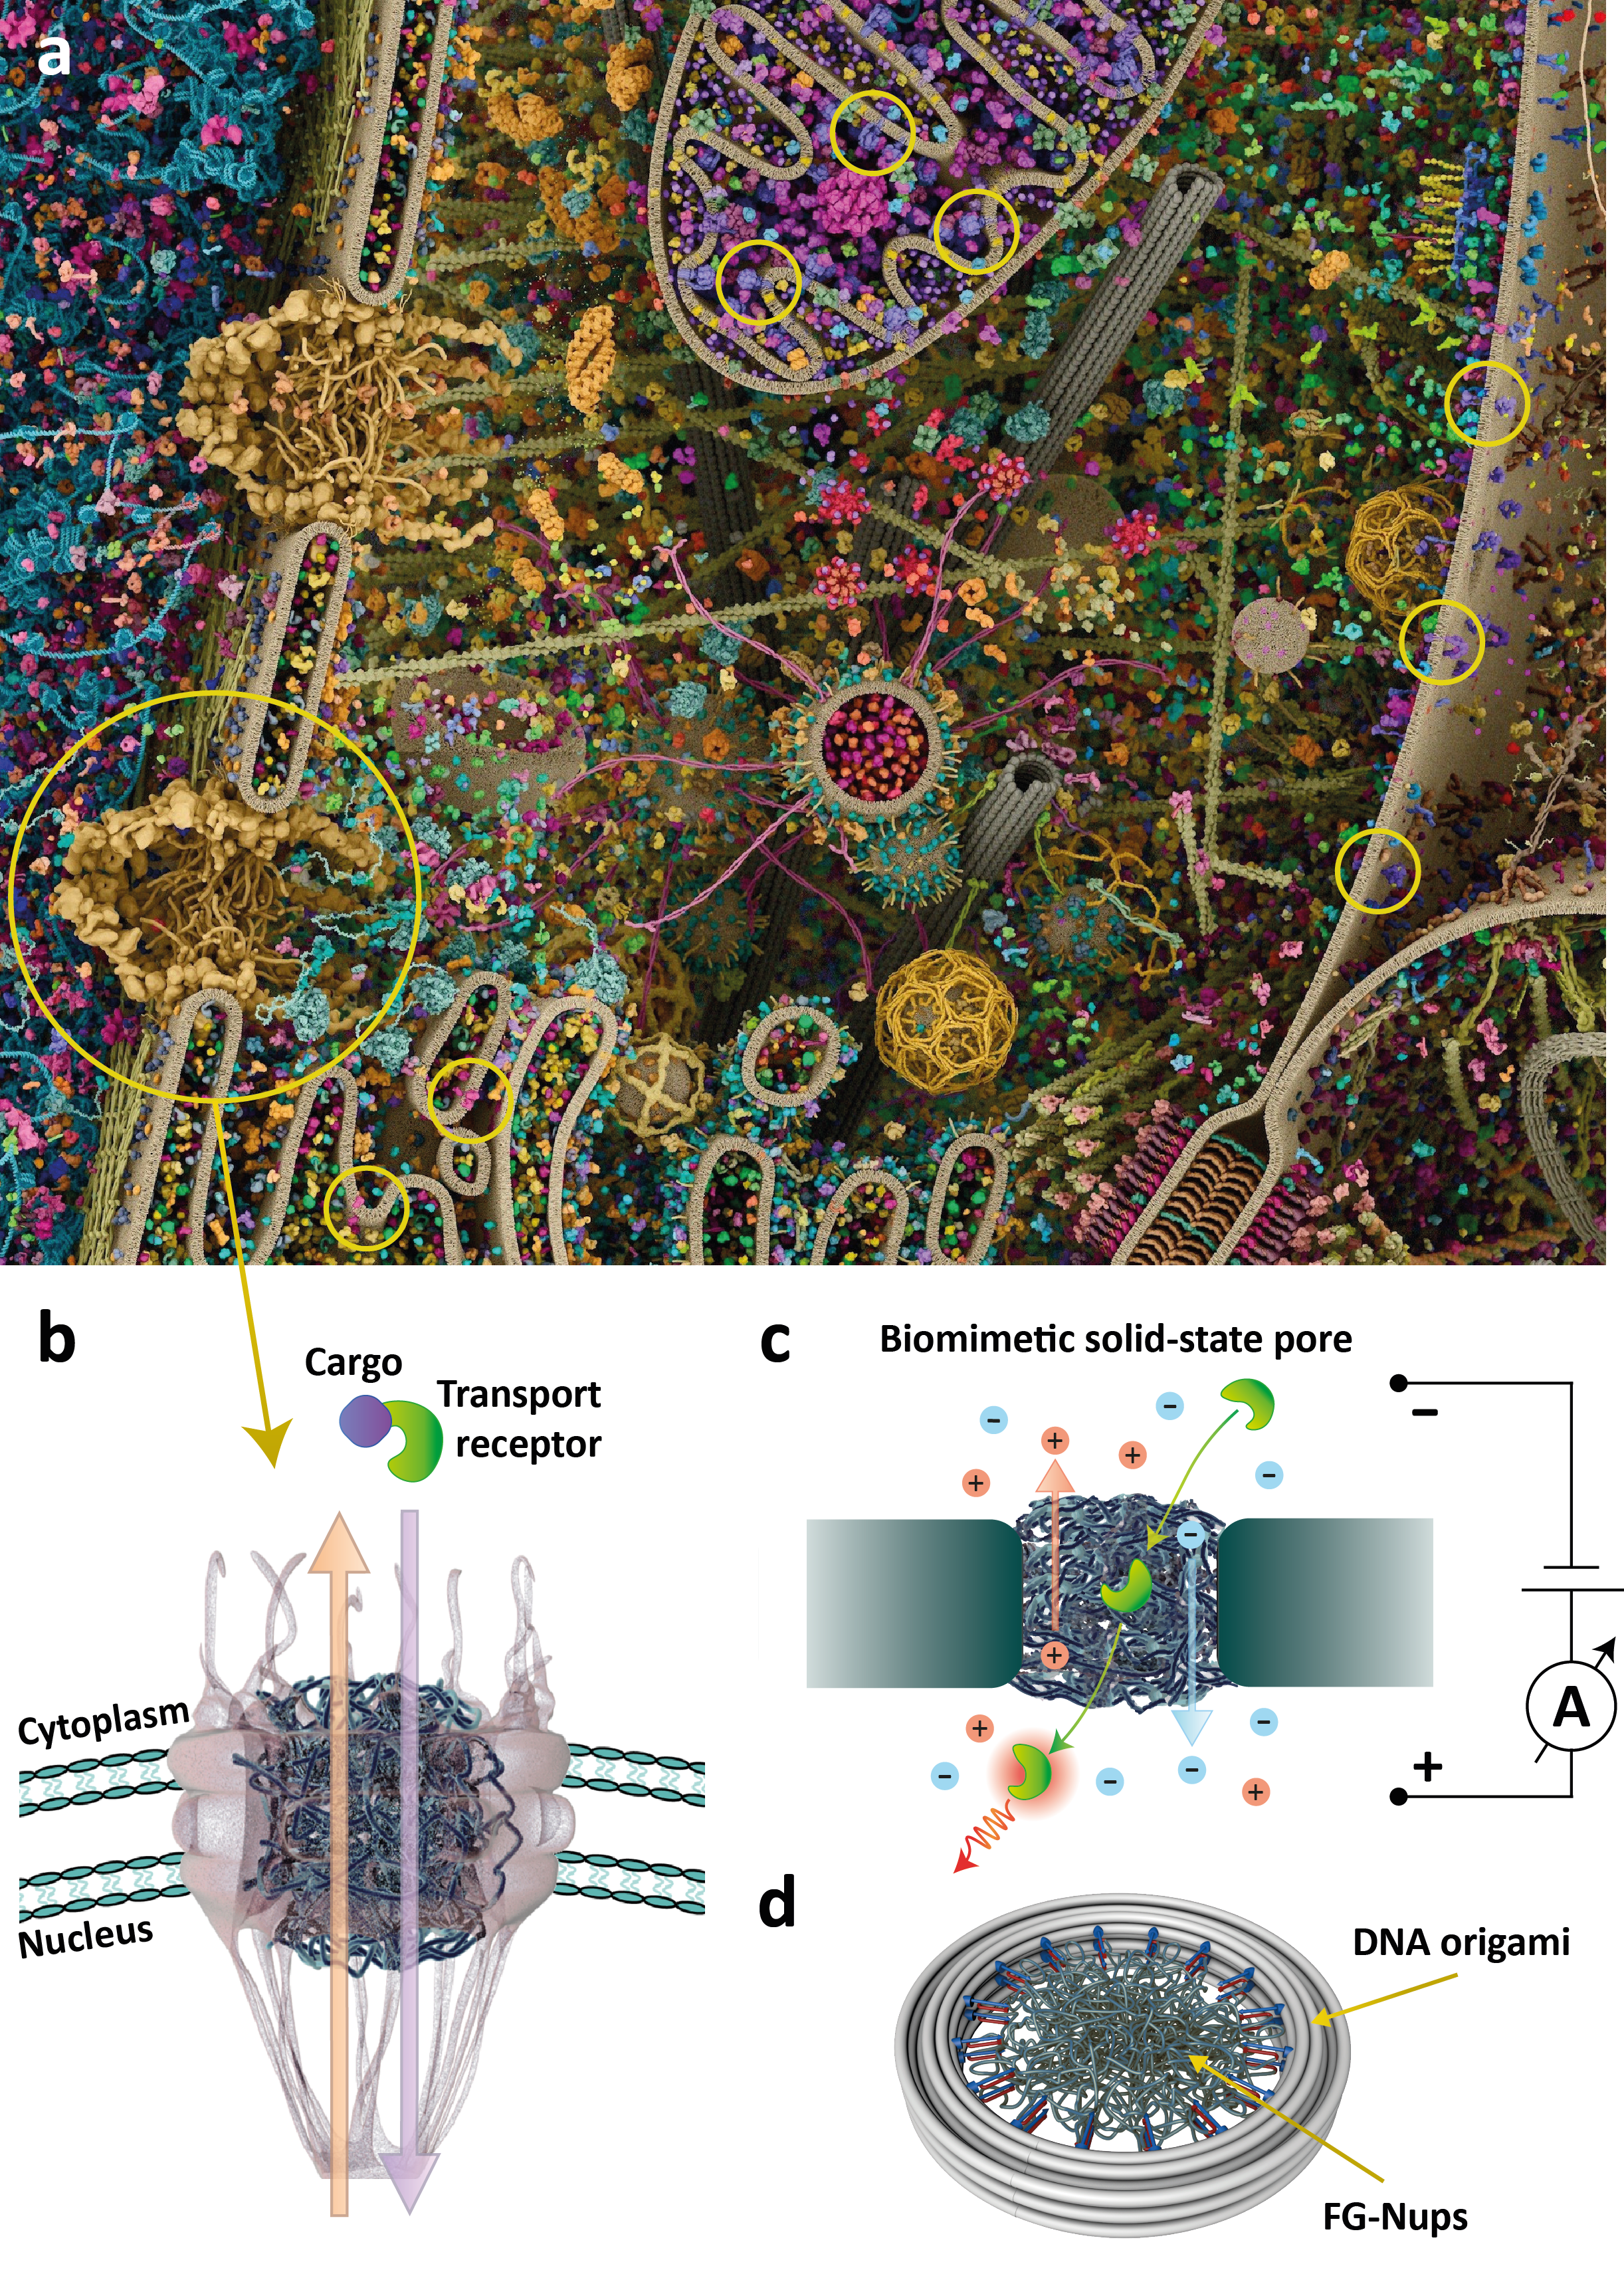
\includegraphics[width=1\linewidth]{figures/Figure6.4.png}
	\caption{a, Sketch of the interior of a eukaryotic cell (adapted from https://gaelmcgill.artstation.com/projects/Pm0JL1). Yellow circles indicate a nuclear pore complex (left) and three mitochondrial pores (right). b, Schematic of the NPC (adapted from https://sites.google.com/site/sspatel/nuclearporecomplex2). The blue filaments represent the FG-Nup mesh. Import (purple) and export (orange) transport pathways are indicated. c, Schematic of a biomimetic solid-state nanopore, where FG-Nups are grafted onto a solid-state nanopore, whereupon transport of biomolecules can be measured electrically or optically. d, Sketch of a biomimetic NPC, built by attaching FG-Nups (blue) to a DNA-origami scaffold (grey).}
	\label{fig:fig6.4}
\end{figure}
This proved for the first time that the FG-Nup mesh alone is sufficient to impart a selective transport barrier – a striking finding considering that the biomimetic NPCs consisted of only 1 type of FG-Nups while native NPCs feature more than 10 different FG-Nups types. Kowalczyk \emph{et al.} \cite{Kowalczyk2011a} measured selective transport across individual biomimetic nanopores, formed by grafting FG-Nups to the inner walls of a solid-state nanopore (Fig. \ref{fig:fig6.4}c), where ion current measurements provided single-molecule resolution. These biomimetic NPCs provided first insights into the FG-Nups conformation within the pore by examining the behavior of the conductance as a function of pore diameter. Follow-up work by Ananth \emph{et al.} \cite{Ananth2018} emphasized the key role of the hydrophobic residues of the FG-Nups, as a mutant where hydrophobic amino acids were replaced by hydrophilic ones lost the selectivity altogether. These experiments, coupled with molecular dynamics simulations, revealed the important role of cohesiveness of the FG-mesh for achieving proper selective behavior. More recently, nanopores functionalized with user-defined protein sequences that mimic native FG-Nups were also shown to be selective, demonstrating the outstanding robustness of FG-Nups to drastic changes in their amino acid sequence \cite{Fragasso2021}. A creative alternative approach to mimic NPCs is the use of a DNA-origami ring as a scaffold with programmable sites for anchoring FG-Nups (Fig. \ref{fig:fig6.4}d) \cite{Ketterer2018,Fisher2018}. This platform was employed for imaging the spatial arrangements of confined FG-Nups using cryo-electron microscopy and atomic force microscopy, and allows the exploration more complex FG-meshes that combine different types of FG-Nups. 


\section[Nanopore sensors for biomarker identification and quantification in clinical samples]{Nanopore sensors for biomarker identification and quantification in clinical samples}
\sectionmark{Nanopore sensors for clinical applications}

The adaptation of nanopore sensing technologies for clinical samples presents new challenges associated with the greater complexity and heterogenous nature of medical specimens, as compared to lab-made samples (Fig. \ref{fig:fig6.5}). Additionally, clinical sensing often requires extremely high precision, specificity, and sensitivity which further complicate its implementation. Nevertheless, the potential ability of nanopores to offer a generic and highly flexible sensing platform for liquid biopsy stands out as a high-impact opportunity that has begun to be addressed only in recent years.


Two primary factors can be identified as the main roadblocks in realizing this vision: First, unlike lab-made `analytical samples', the target biomolecules in clinical samples (often nucleic acids or protein biomarkers) span large range of concentrations from as low as tens of aM ($10^{-18}$ M) for some blood pathogenic infections and circulating tumor DNAs to sub-nM ($10^{-9}$ M) concentrations for SARS, influenza as well as other biomarkers \cite{Kelley2017}. In many cases the super low biomarkers concentration severely limit the use of standard purification/concentration techniques \cite{Galenkamp2018}. Second, most clinical samples contain an abundancy of constituents that may interfere with the nanopore sensor itself (\emph{i.e.} blocking the nanopore or causing false translocation events). In particular, bodily fluids such as plasma, urine, and nasal secretions can clog the nanopore prematurely. At the same time bulk purification assays, including liquid chromatography and `clean-up' columns, that are broadly used in life sciences research, are not optimal for nanopore based single-molecule sensing as they are lossy, time-consuming, and may not transfer well to point-of-care applications.


In recent years researchers have begun to tackle these challenges by developing smart assays and devices for treatment of clinical samples, which take advantage of some of the unique capabilities of nanopore sensors. Particularly, owing to their extremely small and compact form factor, nanopore sensors can be integrated in microfluidic devices serving either sample preparation or analyte concentration, further increasing its yield of detection \cite{Galenkamp2018}. Moreover, biophysical concentration strategies involving for example dielectrophoretic trapping or isotacophoresis focusing can in principle concentrate the target species by several orders of magnitude, and therefore bear potential towards the future development of liquid biopsy applications involving biomolecule-based disease prognostics and diagnostics \cite{Freedman2016,Spitzberg2020}. 


To enhance molecular specificity and circumvent the negative effects of background molecules on nanopore functionality, a number of biochemical assays have already been developed. These assays involve minimal losses of target molecules during the sample preparation while at the same time they protect the nanopore by selective degradation of background molecules. For example, nanopore-based direct, digital counting of single nucleotide polymorphic sites marked with Locked Nucleic Acids synthetic molecules was used for detection of Shiga toxin producing Escherichia coli serotype and cancer-derived driver mutations \cite{Tian2018,Wang2017a}. Another approach utilized the extremely high specificity of DNA ligase to pull-down selected circulating tumor DNA mutations associated with breast cancer genes (\emph{i.e.} ERBB2 and PIK3Ca) in blood samples \cite{Burck2021}. These mutations were sensed optically by tagging the probe oligonucleotides with fluorescent dyes and supplementing the electrical sensing of the nanopore with a single-molecule optical detection approach. In another recent studies the high selectivity of DNA aptamers was used to fabricate specific DNA `carriers' with high affinity for specific protein biomarkers in plasma sample, producing characteristic electrical current traces when translocated through a nanopore formed at the end of glass-pulled pipettes \cite{Sze2017}. 
\begin{figure}[!htbp]
	\centering
	\includegraphics[width=1\linewidth]{figures/Figure6.5.pdf}
	\caption{Adapting nanopore sensing to biological samples and clinical diagnostics. A variety of biomedical samples sources including bodily fluids or tissue biopsies or biological specimen including cell cultures, bacteria and viruses can be harvested in a minimal and non-lossy biochemical treatment for single-molecule sensing with protein or solid-state nanopores. The ultra-small sample volume (\emph{e.g.} $\mu$L or less) required for the analysis lends itself for hands-free assay development utilizing on-chip microfluids and/or magnetic beads. Nanopore sensing may involve either pure electrical digital counting of biomolecules or a combined electro-optical sensing to enhance the system multiplexing ability. Data analysis is supported by advanced machine learning approaches to classify and count the target biomolecules.}
	\label{fig:fig6.5}
\end{figure}
Taking advantage of electro-optical sensing, short hairpin structure oligonucleotide containing fluorophore and quencher moieties (`molecular beacons') were used to mark and identify specific cDNA molecules from human serum and urine, as they were forced through the tip of a nanopipette \cite{Cai2019}.


An alternative strategy for sensing of protein biomarkers in bio-fluids involved the creation of a protein bait antibody connected to a biological nanopore hence serving as a local `trap' for the target protein \cite{Fahie2015,Fahie2015a,Thakur2019a}. Specifically, Fahie and coworkers modified the outer membrane protein G (OmpG) with a short, biotinylated polymer chain that was used as a sensing probe. The binding/unbinding kinetics of several anti-biotin antibodies (including mAb, pAb.1 and pAb.2) were studied in buffered solution of diluted serum. Interestingly the different anti-biotin antibodies showed remarkably different binding/unbinding kinetic rates presumably due to different antibodies size, shape or charge. A similar approach demonstrated by Thakur and Movileanu involved the truncated t-FhuA protein pore, equipped with a short hexapeptide tether, a barnase (Bn) protein receptor and a dodecapeptide adapter. The capture and release events of a protein analyte by the tethered protein bait occur outside the nanopore and are accompanied by uniform current openings, whereas nonspecific pore penetrations by nontarget components of serum, involve irregular current blockades. As a result of this unique peculiarity of the readout between specific protein captures and nonspecific pore penetration events which result in a highly dynamic ion-current signature, this selective sensor could quantitatively sample proteins and potentially provides richer information on the detected analytes than classical immunosorbent assays. 


The $\alpha$-hemolysin protein pore was used to selectively detect microRNAs (miR) mole\-cules hybridized in solution to oligonucleotides probes, allowing the quantification of the miR-155 biomarker from purified plasma samples of lung cancer patients \cite{Wang2011}. Specific binding of the miR to the probe molecules generated long voltage driven unzipping events, that were readily sensed by analyzing the ion current traces \cite{Mathe2004}. More recently, a purifica\-tion-free method for nanopore based digital counting of mRNA expression was demonstrated \cite{Rozevsky2020}. The method involves Reverse Transcription (RT) of the target genes, directly followed by enzymatic degradation of the background molecules with no intermediate purification stages \cite{Rozevsky2020}. The accuracy of the assay relies on designing highly specific RT primers and avoiding PCR amplification, which could lead to erroneous amplification in cases where the clinical sample contains small amounts of the target mRNA biomarker. The method was used to quantify mRNA cancer biomarkers, such as MACC1, as well as for PCR-free sensing of SARS-Cov-2 clinical samples, potentially showing greater accuracy than the gold standard RT-qPCR method \cite{Galenkamp2018,Wang2011}. 


Nanopore sensing of clinical samples is not limited only to nucleic acids and proteins. Recently, Galenkamp and co-workers demonstrated that the cytolysin A (ClyA) nanopore can be used to sense the concentration of metabolites such as glucose and asparagine, directly from bodily fluids (blood, sweat, urine, saliva) \cite{Galenkamp2018}. Glucose-binding protein (GBP) or substrate-binding domain analogous to GBP were used to sense glucose and asparagine molecules, respectively, by inducing shifts in the dwell-time of the open and closed conformations of the probing proteins, as they were lodged in the nanopore. In all the examples provided for nanopore based sensing of clinical biomarkers, the ability to sense multiple species (DNAs, RNAs, metabolites, \emph{etc.}) using the same nanopore is a direct consequence of the single-molecule nature of the technique in which only one molecule is sensed at the time and a dynamical ion current trajectory over time is used as the basis for target multiplexing. This illustrates the great potential nanopore sensing holds for future complex bio-fluids characterization often involving a multitude of biomarkers.



\section{Conclusion and perspectives}
This review outlined diverse nanopore research directions and applications beyond DNA sequencing. Tremendous progress has been made. Specifically, over the past two decades, nanopores have become an essential single-molecule tool in multiple disciplines including chemistry, biophysics, nanoscience, and others. The ongoing refinement of nanopores structures and shapes provide a well-defined confinement for single-molecule reaction catalysis. By taking advantage of designable nanopores at the molecular scale, the protein nanopore reactor is expected to provide a bottom-up approach for in situ production of customized chemicals. The nanopore has also found growing use as a force transducer allowing controlled localization and trapping of a diverse range of biomolecules for single-molecule biophysics studies. Finally, nanopore-based biomedical applications have grown beyond single DNA sequencing and epigenetic modification analyses, and is currently used in diverse fields from sensing molecular biomarkers (proteins, metabolites and nucleic acids) in biofluids, and other biological specimen. Based on the fast growth rate of nanopore applications, it is likely that it may become the prominent future technique in single-molecule \emph{in vitro} diagnostics.


However, challenges remain for nanopores to meet its full potential. For example, in order to uncover the exact chemical compositions of single molecules (\emph{e.g.}, protein, polysaccharides and glycoprotein), improvements in sensing accuracy and temporal resolution will be necessary. Unlike the relatively simple primary structure of the four cano\-nic DNAs nucleobases, many biopolymers are composed of larger number of chemically diverse building blocks. Specifically, proteins consist of 20 different amino-acids, and polysaccharides of 8-10 monosaccharides units. Therefore, nanopores must be rationally tailored to meet the resolution requirement for each application: their sensing volume should be as small to match the size of a single unit of the sensed monomer, but not too small to allow it to smoothly slide through the nanopore under the applied electric field. More important, the nanopore should be optimally sensitive to the chemical or physical properties of the building blocks, producing distinguishable ionic current signatures for each unit. This could be achieved by carefully functionalizing of the pore inner surfaces to manipulate the interactions between the biopolymer moiety and the nanopore, hence providing the required sensitivity and selectivity. 


To achieve this long-term vision joint efforts of multi-disciplinary fields will be required, including engineering of motor proteins to finely control the biopolymers’ translocation rate through the nanopore, as well as molecular dynamic simulations and advanced analysis methods involving machine learning. In parallel with advances in future nanopore designs, the ability to produce large-scale nanopore devices consisting of millions of individual pores on an small footprint, may greatly impact bioinformatics, producing enormous volumes of sensing data at high speeds. The ongoing developments in nanopore-based sensing strategies will also be beneficial for future venturing in the promising field of molecular-based data storage and retrieval, offering new solutions for some of the most pressing challenges in this area.



\references{chapter-6/chapter-6}
